\documentclass[dvipdfmx]{beamer}\usepackage[]{graphicx}\usepackage[]{color}
% maxwidth is the original width if it is less than linewidth
% otherwise use linewidth (to make sure the graphics do not exceed the margin)
\makeatletter
\def\maxwidth{ %
  \ifdim\Gin@nat@width>\linewidth
    \linewidth
  \else
    \Gin@nat@width
  \fi
}
\makeatother

\definecolor{fgcolor}{rgb}{0.345, 0.345, 0.345}
\newcommand{\hlnum}[1]{\textcolor[rgb]{0.686,0.059,0.569}{#1}}%
\newcommand{\hlstr}[1]{\textcolor[rgb]{0.192,0.494,0.8}{#1}}%
\newcommand{\hlcom}[1]{\textcolor[rgb]{0.678,0.584,0.686}{\textit{#1}}}%
\newcommand{\hlopt}[1]{\textcolor[rgb]{0,0,0}{#1}}%
\newcommand{\hlstd}[1]{\textcolor[rgb]{0.345,0.345,0.345}{#1}}%
\newcommand{\hlkwa}[1]{\textcolor[rgb]{0.161,0.373,0.58}{\textbf{#1}}}%
\newcommand{\hlkwb}[1]{\textcolor[rgb]{0.69,0.353,0.396}{#1}}%
\newcommand{\hlkwc}[1]{\textcolor[rgb]{0.333,0.667,0.333}{#1}}%
\newcommand{\hlkwd}[1]{\textcolor[rgb]{0.737,0.353,0.396}{\textbf{#1}}}%
\let\hlipl\hlkwb

\usepackage{framed}
\makeatletter
\newenvironment{kframe}{%
 \def\at@end@of@kframe{}%
 \ifinner\ifhmode%
  \def\at@end@of@kframe{\end{minipage}}%
  \begin{minipage}{\columnwidth}%
 \fi\fi%
 \def\FrameCommand##1{\hskip\@totalleftmargin \hskip-\fboxsep
 \colorbox{shadecolor}{##1}\hskip-\fboxsep
     % There is no \\@totalrightmargin, so:
     \hskip-\linewidth \hskip-\@totalleftmargin \hskip\columnwidth}%
 \MakeFramed {\advance\hsize-\width
   \@totalleftmargin\z@ \linewidth\hsize
   \@setminipage}}%
 {\par\unskip\endMakeFramed%
 \at@end@of@kframe}
\makeatother

\definecolor{shadecolor}{rgb}{.97, .97, .97}
\definecolor{messagecolor}{rgb}{0, 0, 0}
\definecolor{warningcolor}{rgb}{1, 0, 1}
\definecolor{errorcolor}{rgb}{1, 0, 0}
\newenvironment{knitrout}{}{} % an empty environment to be redefined in TeX

\usepackage{alltt}
\usetheme{Boadilla}
%\usepackage{helvet}
\usepackage[dvipdfmx]{graphicx}
\usepackage[dvipdfmx]{color}
\usepackage{float}
\usepackage{standalone}
\usepackage{tikz}
\usepackage{booktabs}
\usepackage{dcolumn} % to align numeric values at decimal mark in stargazer

%\usepackage{geometry}
%\geometry{a4paper,portrait,margin=1in} % graph extended to the defined width. graph size need to be defined in global environment
%\AtBeginSection[] % show highlighted table of contents for each section
%{
%  \begin{frame}
%    \frametitle{Table of Contents}
%    \tableofcontents[currentsection]
%  \end{frame}
%}

\usepackage[backend=bibtex,maxnames=1,sorting=none]{biblatex}
\bibliographystyle{abbrv}
\bibliography{ne_pain.bib}


\title{Neighborhood environment and chronic pain among older adults}
\subtitle{Swedish Annual Level of Living Survey}
\author{Kenta Okuyama\inst{1,2}}
\institute{\inst{1}Center for Primary Health Care Research \\
Lund University\and \inst{2}Center for Community-based Healthcare Research and Education \\
Shimane University}
\date{\today}
\logo{
	
\includegraphics[height=1.0cm]{/home/kenta/Dropbox/research_projects/research_proposal/logo/lund_RGB.png}~
	%\includegraphics[height=1.0cm]{/home/kenta/Dropbox/Logo/logo_shimaneUniv.png}
}

%%%%%%%%%%%%%%%%%%%%%%%%%%%
\IfFileExists{upquote.sty}{\usepackage{upquote}}{}
\begin{document}
\begin{frame}
	\titlepage
\end{frame}

%%%%%%%%%%%%%%%%%%%%%%%%%%%
%\begin{frame}
%	\frame{Table of Contents}
%	\tableofcontents
%\end{frame}

%%%%%%%%%%%%%%%%%%%%%%%%%%%
\section{Introduction - Older adults}
\begin{frame}
	\frametitle{Introduction}
	\begin{itemize}
		\item World population is ageing (UN, 2017) \cite{unitednationsWorldPopulationAgeing2017a}.
			\begin{figure}[H]
				\centering
				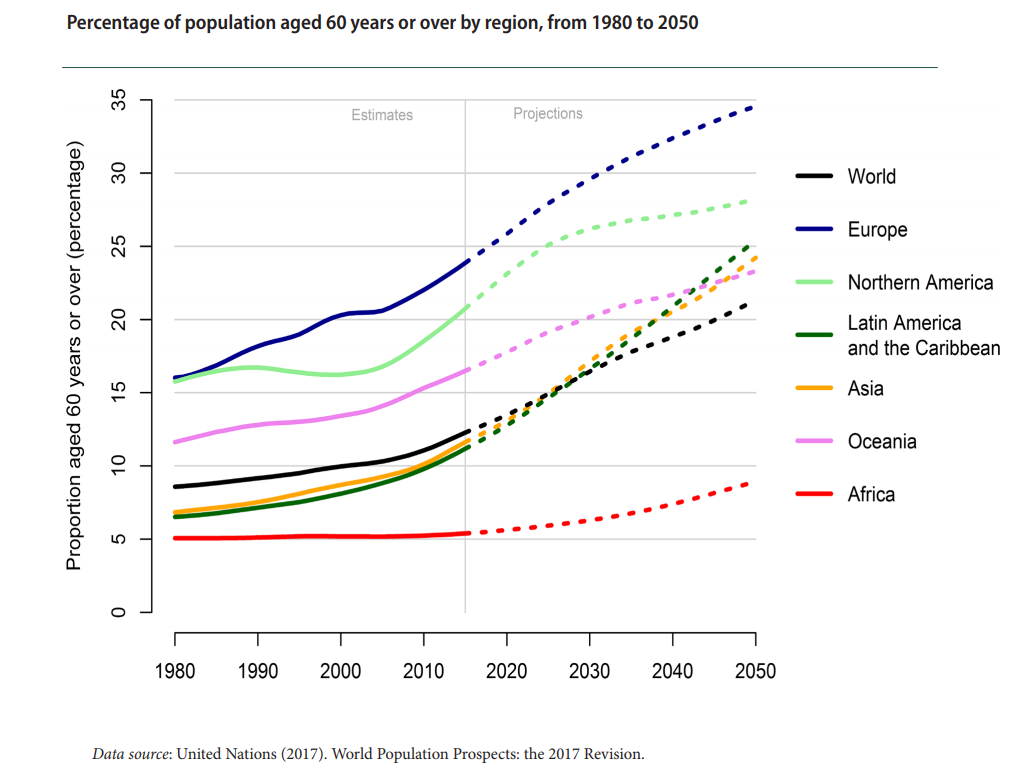
\includegraphics [width=0.8\textwidth, height=0.8\textheight] {./img/pop_ageing.PNG}
			\end{figure}
	\end{itemize}
\end{frame}

%%%%%%%%%%%%%%%%%%%%%%%%%%%
\begin{frame}
	\frametitle{Introduction - Older adults}
	\begin{itemize}
		\item Longer life = more oppotunities \cite{raggiDeterminantsMobilityPopulations2018}
			\begin{itemize}
				\item Seek further careers, educations as individuals.
				\item Valuable contributions to society.
			\end{itemize}
		\item but it depends on.... health.
	\end{itemize}
\end{frame}

%%%%%%%%%%%%%%%%%%%%%%%%%%%
\begin{frame}
	\frametitle{Introduction - Older adults}
	\begin{itemize}
		\item Life expectancy = healthy life expectancy (disability free).
			\begin{figure}[H]
				\centering
				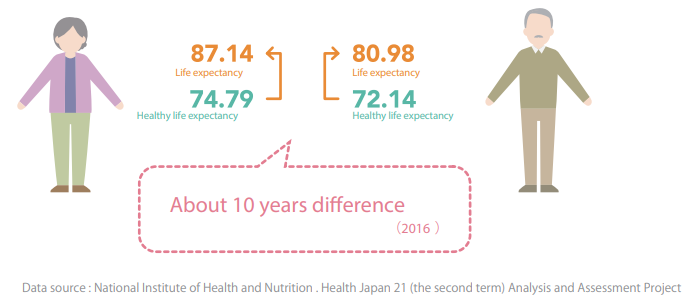
\includegraphics [width=0.8\textwidth, height=0.6\textheight] {img/healthylife_jp.PNG}
			\end{figure}
	\end{itemize}
\end{frame}

%%%%%%%%%%%%%%%%%%%%%%%%%%%
\begin{frame}
	\frametitle{Introduction - Older adults}
	\begin{itemize}
		\item End of healthy life = Lost functional ability and become care-dependent.
		\item Determinants of care dependent = physical disorders, especially from fall. 
		\item Pain, is one of the biggest factor for falls, and even mental health.
			\begin{figure}[H]
				\centering
				\documentclass[dvipdfmx]{article}

\usetikzlibrary{shapes.geometric, arrows}


\begin{document}
    \tikzstyle{heading} = [rectangle, rounded corners, minimum width=3cm, minimum height=1cm,text centered, draw=white]
    \tikzstyle{flow} = [rectangle, rounded corners, minimum width=3cm, minimum height=1cm,text centered, draw=black]

\begin{tikzpicture}[node distance=3cm]

    \node (head1) [text width=4cm] {Number of subjects $\geq$60};
    \node (n0) [flow, below of=head1, text width=5cm, yshift=1cm] {Baseline 2016, n=2724};
    \node (n1)  [flow, below of=n0, text width=5cm] {Follow-up 2017, n=1817};
    \node (n2)  [flow, below of=n1, text width=5cm] {Follow-up 2018, n=1554};
    \node (n3)  [flow, below of=n2, text width=5cm] {Follow-up 2019, n=1200(expected)};

    \node (head2) [text width=4cm, right of=head1, xshift=3cm] {Number of subjects $\geq$60 without missing data for relavant variables};
    \node (n02)  [flow, right of=n0, text width=5cm, xshift=3cm] {Baseline 2016, n=2526};
    \node (n12)  [flow, right of=n1, text width=5cm, xshift=3cm] {Follow-up 2017, n=1565};
    \node (n22)  [flow, right of=n2, text width=5cm, xshift=3cm] {Follow-up 2018, n=1033};
    \node (n32)  [flow, right of=n3, text width=5cm, xshift=3cm] {Follow-up 2019, n=700(expected)};

    \draw [->] (n0) -- node[text width=4cm]{}(n1);
    \draw [->] (n1) -- node[text width=4cm,text centered,fill=white]{baseline and 2017, or baseline only}(n2);
    \draw [->] (n2) -- (n3);
    
    \draw [->] (n02) -- node[text width=4cm]{}(n12);
    \draw [->] (n12) -- node[text width=4cm,text centered,fill=white]{baseline and 2017, or baseline only}(n22);
    \draw [->] (n22) -- (n32);
\end{tikzpicture}   

\end{document}

			\end{figure}
	\end{itemize}
\end{frame}

%%%%%%%%%%%%%%%%%%%%%%%%%%%
\begin{frame}
	\frametitle{Introduction - Pain}
	\begin{itemize}
		\item Fact of pain.
			\begin{itemize}
				\item Pain is a determinant factor for physical function decline.
				\item Associated healthcare cost with pain.
				\item Current issues with pain, mainly treatment.
			\end{itemize}

	\end{itemize}
\end{frame}


%%%%%%%%%%%%%%%%%%%%%%%%%%%
\begin{frame}
	\frametitle{Introduction - Pain and neighborhood} 
	\begin{itemize}
		\item Neighborhood environment
			\begin{itemize}
				\item Some individual risk factors have been found for pain, i.e. SES.
				\item 
			\end{itemize}
	\end{itemize}
\end{frame}


%%%%%%%%%%%%%%%%%%%%%%%%%%%
\section{Objectives}
\begin{frame}
	\frametitle{Objectives}
	\begin{block}{Objectives}
		\begin{itemize}
			\item To investigate whether neighborhood deprivation is associated with chronic pain among older adults.
		\end{itemize}
	\end{block}
	\begin{description}
		\item[Hypothesis] \mbox{}\par
			\begin{itemize} 
				\item Older adults living in deprived areas would have higher risk of having/developing chronic pains.
			\end{itemize} 
		\item[Implication] \mbox{}\par
			\begin{itemize} 
				\item The findings lead to further investigations for what modifiable factors lie in neighborhood deprivation and pain.
			\end{itemize} 
	\end{description}
\end{frame}

%%%%%%%%%%%%%%%%%%%%%%%%%%%
\section{Methods}
\begin{frame}
	\frametitle{Methods - Data source}
	\begin{description}
		\item[Data source] \mbox{}\par
			\begin{itemize} 
				\item Swedish Annual Level of Living Survey
					\begin{itemize}
						\item The Swedish Living Condition Surveys (ULF/SILC).
						\item Started since 1975 ~.
						\item Changed from face-face to phone interviews in 2008 ~.
					\end{itemize} 
			\end{itemize} 
		\item[Study subjects] \mbox{}\par
			\begin{itemize} 
				\item Those who participated in ULF in 2008 - 2013 (3 time points).
				\item Those who participated in ULF in 2014 - 2018 (3 time points).
			\end{itemize} 
	\end{description}

\end{frame}

%%%%%%%%%%%%%%%%%%%%%%%%%%%
\begin{frame}
	\frametitle{Methods - Variables}
	\begin{description}
		\item[Outcome] \mbox{}\par
			\begin{itemize} 
				\item Pain, Severe pain.
					\begin{itemize}
						\item \textbf{2008-2013} Do you suffer from pain? Are the ailments are severe or minor? 1. Back/hips/sciatica, 2. Shoulders/neck, 3. Hands/elbows/legs/knees.
						\item \textbf{2014-2018} Do you suffer from pain? Would you say the ailments are severe or minor? 1. Back/hips, 2. Shoulders/neck, 3. Arms/hands/legs/feet.
					\end{itemize} 
				\item Disease of the musculoskeletal system and connective tissue
					\begin{itemize}
						\item Based on ICD9. From 2012, based on ICD10. 
						\item Ex. Rheumatoid arthritis, osteoarthritis, soft tissue, rheumatism, periostitis.
					\end{itemize} 
				\item Disabilities
					\begin{itemize}
						\item Reduced mobility, motor disability. 
					\end{itemize}
			\end{itemize} 
	\end{description}

\end{frame}



%%%%%%%%%%%%%%%%%%%%%%%%%%%
\begin{frame}
	\frametitle{Methods - Variables}
	\resizebox{\textwidth}{!}{
		\begin{tabular}{ c l p{5cm} }
			\hline
			Type & Name & Description\\
			\hline \hline
			Outcome & Serious/Severe pain & Do you suffer from pain? Would you say the ailments are severe or minor? (2014~2018) Are the ailments are severe or minor? (2008~2013). \\
			Primary exposure & Neighborhood deprivation index & Linked with the measures by SAMS.\\
			Covariates & Basic characteristics & Age, gender, immigration status. \\
								 & Socio-economic status & Education, occupation, marital status, income.\\
								 & Physical activity & Frequencies of leisure time activities, i.e. walking, outdoor sports.\\
								 & Mental conditions & Problems of anxiety, worry, fear.\\
								 & Social relations & Living alone, social contact, time, have friends.\\
								 \hline
		\end{tabular}
	}
\end{frame}

%%%%%%%%%%%%%%%%%%%%%%%%%%%
\begin{frame}
	\frametitle{References}
	
	\printbibliography

\end{frame}

\end{document}
